\documentclass[handouts]{beamer}
\usepackage[orientation=portrait,size=a4, scale=2]{beamerposter}
\beamertemplatenavigationsymbolsempty

\usepackage[czech]{babel}
\usepackage{booktabs}

\title{Lov populace}
\author{Robert Mařík}
\usetheme{CambridgeUS}
\usecolortheme{crane}


\begin{document}

\begin{frame}

  \begin{center}
    \large Lov populace
  \end{center}

  Lov typicky modelujeme jako rozdíl dvou faktorů. Jeden souvisí s růstem populace a druhý se strategií a způsobem lovu. Zajímá nás, zda je populace ohroženy vyhynutím a jaký je výnos lovu.

\begin{itemize}
\item Ve stacionárním bodě je rychlost růstu rovna rychlosti lovu. 
\item Na obrázcích stacionární body vidíme jako průsečík křivek. Na intervalech, kde je
  lov intenzivnější než růst, dochází k poklesu populace.
\item Pokud je pro malé populace lov intenzivnější než růst, populace zanikne.  (první a třetí model)
\item Stabilní stacionární body jsou takové, ve kterých se při malém zakolísání populace směrem dolů nebo nahoru obnovuje předchozí stav. 
\end{itemize}
\everymath{\displaystyle} 

\begin{tabular}{p{5cm}p{7.5cm}
  p{5.5cm}}
  \toprule
  Model & Graf rychlostí růstu a lovu & Popis chování modelu\\
  \midrule
  {\textbf{Lov konstantní rychlostí} \par\bigskip
  $
  \frac{\mathrm dx}{\mathrm dt}=rx\left(1-\frac xK\right)-h
  $}
        &\vtop{\kern -10 pt \hbox to 0 pt{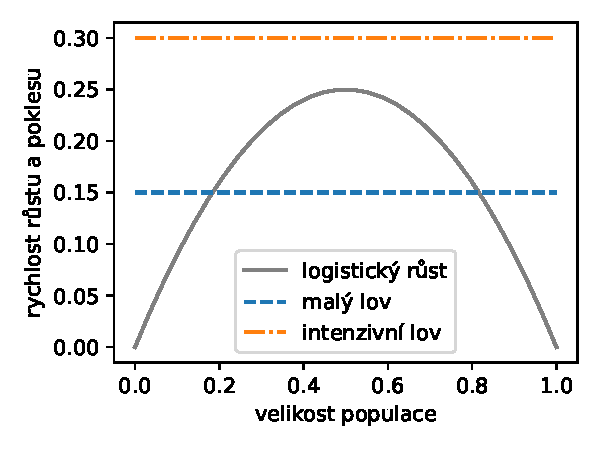
\includegraphics[width=7.3cm]{log_konst.pdf}\hss}}
                         & {V závislosti na $h$ žádný nebo dva kladné stacionární body. Pro malé $h$ je dolní stacionární bod nestabilní a horní stabilní. \par Vzdálenost mezi stacionárními body udává schopnost populace odolávat výkyvům beze změny strategie nebo intenzity lovu. \par Pro malé velikosti populace vymře. \par }
  \\[-10pt]
  {\textbf{Lov konstantním úsilím}  \par\bigskip
  $\frac{\mathrm dx}{\mathrm dt}=rx\left(1-\frac xK\right)-hx$}
        &
          \vtop{\kern -10 pt \hbox to 0 pt{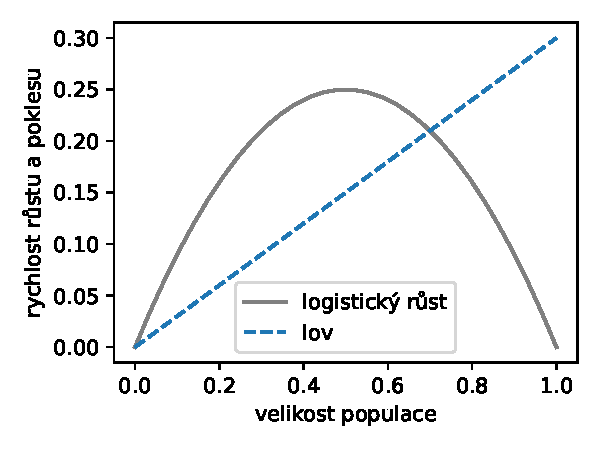
\includegraphics[width=7.3cm]{log_konst_usili.pdf}\hss}}
& Jeden stabilní nenulový stacionární bod. Počátek je nestabilním stacionárním bodem, malá populace vždy roste, populace nevymře.
                                                                 \\[-10pt]
  {\textbf{Lov konstantním úsilím pro populaci s Alleeho efektem}  \par\bigskip
  $\frac{\mathrm dx}{\mathrm dt}=rx^k\left(1-\frac xK\right)-hx$}
        &
          \vtop{\kern -10 pt \hbox to 0 pt{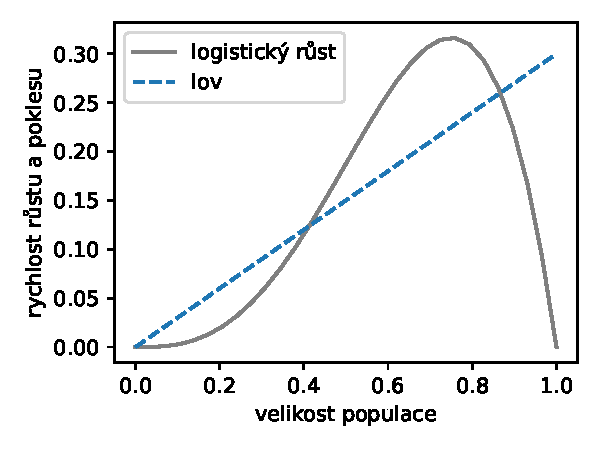
\includegraphics[width=7.3cm]{log_konst_usili_allee.pdf}\hss}}
& Tři stacionární body. Prostřední je nestabilní a odděluje oblasti atraktivity dvou stabilních stacionárních bodů. Jeden stacionární bod (počátek) reprezentuje vymření populace, druhý (vpravo) odpovídá trvale udržitelnému lovu.
                                                                 \\
    \bottomrule
\end{tabular}

\bigskip V obrázcích je vždy $K=1$. V obrázku s Alleeho efektem
hodnota $r$ kompenzuje použitou mocninu, jinak je $r=1$. Tedy velikost
populace měříme v násobcích nosné kapacity prostředí a jednotka času
je taková, že bez započtení konkurence je rychlost růstu populace bez
lovu rovna jedné. Tedy jednotkou času je doba, za jakou by při této rychlosti populace dorostla do své nosné kapacity.

Výnos z lovu pro všechny modely je dán tím, jak vysoko je stabilní
stacionární bod. Bohužel, pokud se snažíme lov nastavit tak, aby
průsečík byl co nejvýše, nutně v případě existence rizika vyhynutí  (první a třetí graf) zužujeme vzdálenost mezi
stabilním a nestabilním stacionárním bodem a zužujeme zónu, ve které
se populace je schopna vyrovnat se zakolísáními sama, bez vnějšího
zásahu.


\end{frame}
\end{document}


%%% Local Variables: 
%%% TeX-command-extra-options: "-shell-escape"
%%% TeX-engine: xetex
%%% End:
